\documentclass{article}
\usepackage[utf8]{inputenc}
\usepackage[vietnamese,english]{babel}
\usepackage{times}
\usepackage{amsmath,amssymb}
\usepackage{tabularx}
\usepackage{array}
\usepackage{booktabs}
\usepackage{graphicx}
\usepackage{xcolor}
\usepackage[
  paperwidth=29.7cm,
  paperheight=16.706cm,
  top=1.0cm,
  bottom=1.0cm,
  left=1.2cm,
  right=1.2cm,
  footskip=0pt,
  headheight=0pt,
  headsep=0pt
]{geometry}

\pagestyle{empty}
\setlength{\parindent}{0pt}
\setlength{\parskip}{0pt}

% Định nghĩa màu sắc thương hiệu
\definecolor{brandGreen}{RGB}{46, 125, 50}
\definecolor{brandRed}{RGB}{211, 47, 47}
\definecolor{brandBlue}{RGB}{21, 101, 192}

\begin{document}
\selectlanguage{vietnamese}

% ==============================================================================
% SLIDE 1: TRANG TIÊU ĐỀ
% ==============================================================================
\begin{center}
\vspace*{0.6cm}
{\fontsize{24}{30}\selectfont \textbf{TRUNG TÂM LUYỆN THI HÓA HỌC THẦY THẠNH}}\\[0.6cm]
{\fontsize{34}{42}\selectfont \textbf{\color{brandGreen}ĐỀ KIỂM TRA 40 PHÚT -- ĐỀ SỐ 04}}\\[0.4cm]
{\fontsize{28}{36}\selectfont \textbf{MÔN: HÓA HỌC 10 -- NỘI DUNG: CHƯƠNG 1, 2}}\\[0.8cm]
{\fontsize{22}{30}\selectfont \textit{Cho biết nguyên tử khối: H = 1; C = 12; N = 14; O = 16; Na = 23; Mg = 24; Al = 27;}}\\[0.2cm]
{\fontsize{22}{30}\selectfont \textit{S = 32; Cl = 35,5; K = 39; Ca = 40; Fe = 56; Cu = 64; Ag = 108; Ba = 137.}}\\[1.0cm]
{\fontsize{24}{30}\selectfont \textbf{\color{brandRed}Thầy TRẦN VĂN THẠNH -- 0777.470.803}}\\[0.3cm]
{\fontsize{20}{26}\selectfont CS1: 6/15 Nguyễn Hoàng, P. Kim Long, TP Huế \quad | \quad CS2: 24 Đặng Thái Thân, TP Huế}
\end{center}
\newpage

% ==============================================================================
% PHẦN I. CÂU TRẮC NGHIỆM NHIỀU PHƯƠNG ÁN LỰA CHỌN (2 CÂU / SLIDE - 30PT)
% ==============================================================================

% SLIDE 2: CÂU 1 & CÂU 2
\fontsize{30}{39}\selectfont
\textbf{Câu 1.} Nguyên tố R có số hiệu nguyên tử bằng 25. Vị trí của R trong bảng tuần hoàn là
\vspace{8pt}

\begin{tabularx}{\linewidth}{@{}X X@{}}
\textbf{A.} chu kì 4, nhóm VB. & \textbf{B.} chu kì 4, nhóm VIIA.\\[8pt]
\textbf{C.} chu kì 4, nhóm VIIB. & \textbf{D.} chu kì 4, nhóm IIA.
\end{tabularx}

\vspace*{\fill}

\textbf{Câu 2.} Nguyên tử của nguyên tố X có tổng số hạt là 52. Trong đó, tổng số hạt mang điện nhiều hơn số hạt không mang điện là 16. Kí hiệu nguyên tử của X là
\vspace{8pt}

\begin{tabularx}{\linewidth}{@{}X X@{}}
\textbf{A.} $_{16}^{36}\text{X}$. & \textbf{B.} $_{18}^{34}\text{X}$.\\[8pt]
\textbf{C.} $_{17}^{37}\text{X}$. & \textbf{D.} $_{17}^{35}\text{X}$.
\end{tabularx}
\vspace*{\fill}
\newpage

% SLIDE 3: CÂU 3 & CÂU 4
\fontsize{30}{39}\selectfont
\textbf{Câu 3.} Nguyên tử nguyên tố X có $Z = 17$. X có số lớp electron là
\vspace{8pt}

\begin{tabularx}{\linewidth}{@{}X X@{}}
\textbf{A.} 4. & \textbf{B.} 1.\\[8pt]
\textbf{C.} 2. & \textbf{D.} 3.
\end{tabularx}

\vspace*{\fill}

\textbf{Câu 4.} X là nguyên tố nhóm IIIA. Công thức oxide ứng với hóa trị cao nhất của X là
\vspace{8pt}

\begin{tabularx}{\linewidth}{@{}X X@{}}
\textbf{A.} $\text{X}_2\text{O}$. & \textbf{B.} $\text{XO}_2$.\\[8pt]
\textbf{C.} $\text{XO}$. & \textbf{D.} $\text{X}_2\text{O}_3$.
\end{tabularx}
\vspace*{\fill}
\newpage

% SLIDE 4: CÂU 5 & CÂU 6
\fontsize{30}{39}\selectfont
\textbf{Câu 5.} Nguyên tố hóa học là tập hợp các nguyên tử có cùng
\vspace{8pt}

\begin{tabularx}{\linewidth}{@{}X X@{}}
\textbf{A.} khối lượng. & \textbf{B.} số khối.\\[8pt]
\textbf{C.} số neutron. & \textbf{D.} điện tích hạt nhân.
\end{tabularx}

\vspace*{\fill}

\textbf{Câu 6.} Electron thuộc lớp nào sau đây liên kết với hạt nhân chặt chẽ nhất?
\vspace{8pt}

\begin{tabularx}{\linewidth}{@{}X X@{}}
\textbf{A.} Lớp N. & \textbf{B.} Lớp K.\\[8pt]
\textbf{C.} Lớp L. & \textbf{D.} Lớp M.
\end{tabularx}
\vspace*{\fill}
\newpage

% SLIDE 5: CÂU 7 & CÂU 8
\fontsize{30}{39}\selectfont
\textbf{Câu 7.} Nguyên tử O có 8 electron. Biểu diễn sự sắp xếp electron trong nguyên tử O theo orbital nào sau đây là đúng?
\vspace{6pt}

\begin{tabularx}{\linewidth}{@{}X X@{}}
\textbf{A.} \raisebox{-0.35\height}{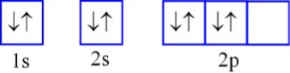
\includegraphics[height=1.55cm]{images_hoa10_de04/image5.png}} & \textbf{B.} \raisebox{-0.35\height}{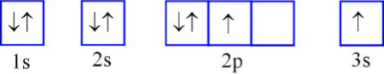
\includegraphics[height=1.55cm]{images_hoa10_de04/image6.png}}\\[12pt]
\textbf{C.} \raisebox{-0.35\height}{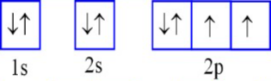
\includegraphics[height=1.55cm]{images_hoa10_de04/image7.png}} & \textbf{D.} \raisebox{-0.35\height}{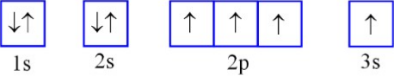
\includegraphics[height=1.55cm]{images_hoa10_de04/image8.png}}
\end{tabularx}

\vspace*{\fill}

\textbf{Câu 8.} Nguyên tử của nguyên tố nào sau đây có tính phi kim mạnh nhất? Cho biết nguyên tố này có trong thành phần của hợp chất teflon, được sử dụng để tráng chảo chống dính.
\vspace{6pt}

\begin{tabularx}{\linewidth}{@{}X X@{}}
\textbf{A.} Phosphorus. & \textbf{B.} Fluorine.\\[8pt]
\textbf{C.} Bromine. & \textbf{D.} Iodine.
\end{tabularx}
\vspace*{\fill}
\newpage

% SLIDE 6: CÂU 9 & CÂU 10
\fontsize{30}{39}\selectfont
\textbf{Câu 9.} Đại lượng đặc trưng cho khả năng hút electron của nguyên tử các nguyên tố khi hình thành liên kết hoá học là
\vspace{8pt}

\begin{tabularx}{\linewidth}{@{}X X@{}}
\textbf{A.} độ âm điện. & \textbf{B.} bán kính nguyên tử.\\[8pt]
\textbf{C.} số hiệu nguyên tử. & \textbf{D.} điện tích hạt nhân.
\end{tabularx}

\vspace*{\fill}

\textbf{Câu 10.} Các hạt cấu tạo nên hầu hết các nguyên tử là
\vspace{8pt}

\begin{tabularx}{\linewidth}{@{}X X@{}}
\textbf{A.} electron, neutron và proton. & \textbf{B.} electron và neutron.\\[8pt]
\textbf{C.} neutron và proton. & \textbf{D.} electron và proton.
\end{tabularx}
\vspace*{\fill}
\newpage

% SLIDE 7: CÂU 11 & CÂU 12
\fontsize{30}{39}\selectfont
\textbf{Câu 11.} Sulfur dạng kem bôi được sử dụng để điều trị mụn trứng cá. Nguyên tử sulfur có phân lớp electron ngoài cùng là $3\text{p}^4$. Phát biểu nào sau đây \textbf{không} đúng khi nói về nguyên tử sulfur?
\vspace{6pt}

\begin{tabularx}{\linewidth}{@{}X X@{}}
\textbf{A.} Sulfur nằm ở chu kì 3. & \textbf{B.} Sulfur nằm ở nhóm VIA.\\[8pt]
\textbf{C.} Hạt nhân nguyên tử S có 16 electron. & \textbf{D.} Lớp ngoài cùng của S có 6 electron.
\end{tabularx}

\vspace*{\fill}

\textbf{Câu 12.} Số electron tối đa chứa trong các phân lớp s, p, d, f lần lượt là
\vspace{8pt}

\begin{tabularx}{\linewidth}{@{}X X@{}}
\textbf{A.} 2, 6, 10, 14. & \textbf{B.} 2, 8, 18, 32.\\[8pt]
\textbf{C.} 2, 4, 6, 8. & \textbf{D.} 2, 6, 8, 18.
\end{tabularx}
\vspace*{\fill}
\newpage

% SLIDE 8: CÂU 13 & CÂU 14
\fontsize{30}{39}\selectfont
\textbf{Câu 13.} Cho X, Y, Z, T là các nguyên tố khác nhau trong số bốn nguyên tố: $_{11}\text{Na}$, $_{12}\text{Mg}$, $_{13}\text{Al}$, $_{19}\text{K}$ và bán kính nguyên tử (nm): $\text{X} = 0,125$; $\text{Y} = 0,203$; $\text{Z} = 0,136$; $\text{T} = 0,157$. Nhận xét nào sau đây là đúng?
\vspace{6pt}

\begin{tabularx}{\linewidth}{@{}X X@{}}
\textbf{A.} X là Na, Y là K. & \textbf{B.} Z là Al, T là Mg.\\[8pt]
\textbf{C.} X là Na, Z là Al. & \textbf{D.} Y là K, T là Na.
\end{tabularx}

\vspace*{\fill}

\textbf{Câu 14.} Có bao nhiêu nguyên tố mà nguyên tử của nó có phân lớp electron lớp ngoài cùng là $4\text{s}^1$?
\vspace{8pt}

\begin{tabularx}{\linewidth}{@{}X X@{}}
\textbf{A.} 3. & \textbf{B.} 1.\\[8pt]
\textbf{C.} 7. & \textbf{D.} 8.
\end{tabularx}
\vspace*{\fill}
\newpage

% SLIDE 9: CÂU 15 & CÂU 16
\fontsize{30}{39}\selectfont
\textbf{Câu 15.} Nguyên tố X tham gia vào hơn 300 phản ứng sinh học và là vi chất quan trọng thứ 4 trong cơ thể con người. Nguyên tử của nguyên tố X có 3 lớp electron và trên lớp thứ 3 chứa 2 electron. Cấu hình electron và tính chất của X là
\vspace{6pt}

\begin{tabularx}{\linewidth}{@{}X X@{}}
\textbf{A.} $1\text{s}^2 2\text{s}^2 2\text{p}^6 3\text{s}^2$, phi kim. & \textbf{B.} $1\text{s}^2 2\text{s}^2 2\text{p}^6 3\text{s}^2$, kim loại.\\[8pt]
\textbf{C.} $1\text{s}^2 2\text{p}^6 3\text{s}^2 3\text{p}^2$, kim loại. & \textbf{D.} $1\text{s}^2 2\text{s}^2 2\text{p}^6 3\text{s}^2 3\text{p}^2$, phi kim.
\end{tabularx}

\vspace*{\fill}

\textbf{Câu 16.} Lớp electron có số electron tối đa gọi là lớp electron bão hòa. Tổng số electron tối đa có trong lớp M là
\vspace{8pt}

\begin{tabularx}{\linewidth}{@{}X X@{}}
\textbf{A.} 18. & \textbf{B.} 10.\\[8pt]
\textbf{C.} 8. & \textbf{D.} 32.
\end{tabularx}
\vspace*{\fill}
\newpage

% SLIDE 10: CÂU 17 & CÂU 18
\fontsize{23}{29}\selectfont
\textbf{Câu 17.} Phát biểu nào dưới đây \textbf{không} đúng?
\vspace{2pt}

\textbf{A.} Hạt nhân nguyên tử được cấu thành từ các hạt proton và neutron.\\
\textbf{B.} Nguyên tử có cấu trúc đặc khít, gồm vỏ nguyên tử và hạt nhân nguyên tử.\\
\textbf{C.} Vỏ nguyên tử được cấu thành bởi các hạt electron.\\
\textbf{D.} Nguyên tử được cấu thành từ các hạt cơ bản là proton, neutron và electron.

\vspace*{\fill}

\textbf{Câu 18.} Phát biểu nào sau đây \textbf{không} đúng?
\vspace{2pt}

\textbf{A.} Nguồn năng lượng được coi như vô tận đối với loài người là năng lượng từ Mặt Trời.\\
\textbf{B.} Các chất hóa học có trong mọi thứ xung quanh ta như lương thực -- thực phẩm, nhiên liệu, nguyên liệu, vật liệu để sản xuất, các loại thuốc chữa bệnh, \dots\\
\textbf{C.} Mỗi năm, hàng triệu tấn các hóa chất cơ bản như sulfuric acid, ammonia, phân bón, chất dẻo, \dots được sản xuất để phục vụ nhu cầu của đời sống và công nghiệp.\\
\textbf{D.} Hóa học chỉ có ứng dụng trong sản xuất hóa chất và trồng trọt.
\vspace*{\fill}
\newpage

% ==============================================================================
% PHẦN II. CÂU TRẮC NGHIỆM ĐÚNG SAI (1 CÂU / SLIDE - 26PT)
% ==============================================================================

% SLIDE 11: PHẦN II - CÂU 1
\fontsize{26}{34}\selectfont
\textbf{Câu 1 (Phần II).} Calcium (Ca) là nguyên tố giúp xương chắc khỏe, phòng ngừa bệnh loãng xương, biết calcium có số hiệu nguyên tử là 20.
\vspace{16pt}

a) Ca thuộc ô số 20, chu kì 3, nhóm IIA. \hfill $[\quad]$\\[14pt]
b) Ca là nguyên tố s. \hfill $[\quad]$\\[14pt]
c) Cấu hình electron của Ca là $1\text{s}^2 2\text{s}^2 2\text{p}^6 3\text{s}^2 3\text{p}^6 4\text{s}^2$. \hfill $[\quad]$\\[14pt]
d) Bán kính nguyên tử của Ca lớn hơn so với bán kính nguyên tử của Mg ($Z=12$). \hfill $[\quad]$
\vspace*{\fill}
\newpage

% SLIDE 12: PHẦN II - CÂU 2
\fontsize{24}{30}\selectfont
\begin{minipage}[c]{0.62\linewidth}
\textbf{Câu 2 (Phần II).} Khi nghiên cứu về sự chuyển động của electron trong nguyên tử có các mô hình như hình bên.\\[6pt]
a) Theo Rutherford -- Bohr, các electron chuyển động xung quanh hạt nhân theo những quỹ đạo xác định. Theo mô hình hiện đại, trong nguyên tử, electron chuyển động rất nhanh, không theo quỹ đạo xác định. \hfill $[\quad]$\\[6pt]
b) Khái niệm ``orbital nguyên tử'' mô tả vùng không gian có xác suất tìm thấy electron lớn nhất, xuất phát từ mô hình Rutherford -- Bohr. \hfill $[\quad]$\\[6pt]
c) Trong cùng một nguyên tử, electron ở càng xa hạt nhân thì có năng lượng càng cao. \hfill $[\quad]$\\[6pt]
d) Electron s chuyển động trong orbital có hình cầu, electron p chuyển động trong orbital có hình số tám nổi. \hfill $[\quad]$
\end{minipage}\hfill
\begin{minipage}[c]{0.35\linewidth}
\centering
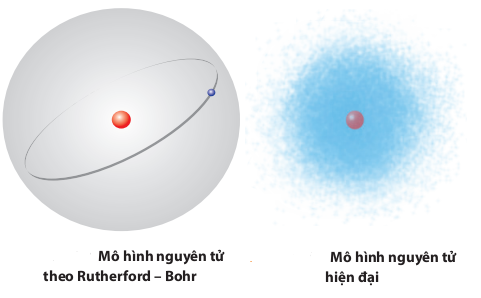
\includegraphics[width=\linewidth]{images_hoa10_de04/image9.png}
\end{minipage}
\vspace*{\fill}
\newpage

% SLIDE 13: PHẦN II - CÂU 3
\fontsize{26}{34}\selectfont
\textbf{Câu 3 (Phần II).} X được làm vỏ phủ vệ tinh nhân tạo hay khí cầu nhằm tăng nhiệt độ nhờ có tính hấp thụ bức xạ điện từ mặt trời khá tốt. Y là một trong những thành phần điều chế nước Javel tẩy trắng quần áo, sợi vải. Nguyên tử nguyên tố X có tổng số hạt electron trong các phân lớp p là 7. Số hạt mang điện của một nguyên tử Y nhiều hơn một nguyên tử X là 8 hạt.
\vspace{14pt}

a) Nguyên tử X và nguyên tử Y đều có 3 lớp electron. \hfill $[\quad]$\\[12pt]
b) Tổng số hạt mang điện trong nguyên tử nguyên tố Y là 26. \hfill $[\quad]$\\[12pt]
c) Nguyên tố X có điện tích hạt nhân là $+13$. \hfill $[\quad]$\\[12pt]
d) Nguyên tố X là phi kim, nguyên tố Y là kim loại. \hfill $[\quad]$
\vspace*{\fill}
\newpage

% SLIDE 14: PHẦN II - CÂU 4
\fontsize{26}{34}\selectfont
\textbf{Câu 4 (Phần II).} Cho 3 nguyên tử: $_{17}^{35}\text{X}$, $_{20}^{40}\text{Y}$, $_{17}^{37}\text{Z}$.
\vspace{16pt}

a) X và Z là 2 đồng vị của cùng một nguyên tố hoá học. \hfill $[\quad]$\\[14pt]
b) Số neutron của Y nhiều hơn số neutron của Z là 3. \hfill $[\quad]$\\[14pt]
c) Trong hạt nhân nguyên tử Y, số hạt mang điện nhiều gấp hai lần số hạt không mang điện. \hfill $[\quad]$\\[14pt]
d) X có 7 electron hoá trị. \hfill $[\quad]$
\vspace*{\fill}
\newpage

% ==============================================================================
% PHẦN III. CÂU TRẮC NGHIỆM TRẢ LỜI NGẮN (1 CÂU / SLIDE - 32PT)
% ==============================================================================

% SLIDE 15: PHẦN III - CÂU 1
\fontsize{32}{42}\selectfont
\textbf{Câu 1 (Phần III).} Nguyên tố Y thuộc ở chu kì 3, nhóm VIA trong bảng tuần hoàn. Số hiệu nguyên tử của Y là bao nhiêu?
\vspace{20pt}

\textbf{Trả lời:} $\dots\dots\dots\dots\dots\dots\dots\dots\dots\dots$
\vspace*{\fill}
\newpage

% SLIDE 16: PHẦN III - CÂU 2
\fontsize{32}{42}\selectfont
\textbf{Câu 2 (Phần III).} Cho các nguyên tố có số hiệu nguyên tử lần lượt là 10, 3, 16, 19, 25. Số nguyên tố kim loại là bao nhiêu?
\vspace{20pt}

\textbf{Trả lời:} $\dots\dots\dots\dots\dots\dots\dots\dots\dots\dots$
\vspace*{\fill}
\newpage

% SLIDE 17: PHẦN III - CÂU 3 (Câu 4 đầu trong đề gốc - Phổ khối Neon)
\fontsize{24}{30}\selectfont
\begin{minipage}[c]{0.60\linewidth}
\textbf{Câu 3 (Phần III).} Phổ khối lượng (MS: Mass Spectrum) chủ yếu được sử dụng để xác định phân tử khối, nguyên tử khối của các chất và hàm lượng các đồng vị bền của một nguyên tố. Phổ khối của neon được biểu diễn như Hình 3.5.\\[4pt]
Trục tung biểu thị hàm lượng phần trăm về số nguyên tử của từng đồng vị, trục hoành biểu thị tỉ số $m/z$ (điện tích $z$ của các ion đồng vị neon đều bằng $1+$). Tính nguyên tử khối trung bình của Neon (làm tròn kết quả đến hàng phần mười).\\[6pt]
\textbf{Trả lời:} $\dots\dots\dots\dots\dots\dots\dots\dots\dots\dots$
\end{minipage}\hfill
\begin{minipage}[c]{0.37\linewidth}
\centering
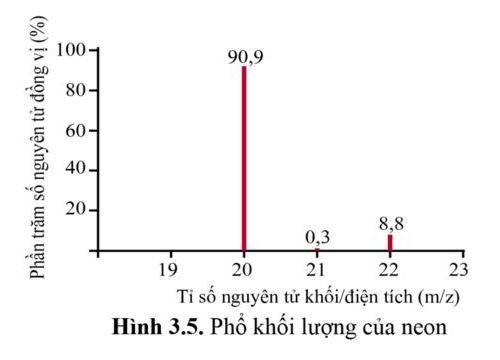
\includegraphics[width=\linewidth]{images_hoa10_de04/hinh_3_5_neon.png}
\end{minipage}
\vspace*{\fill}
\newpage

% SLIDE 18: PHẦN III - CÂU 4
\fontsize{28}{37}\selectfont
\textbf{Câu 4 (Phần III).} Nguyên tử nguyên tố R có cấu hình electron phân lớp ngoài cùng là $2\text{p}^3$, biết nguyên tử khối của R là $15\text{ amu}$.
\vspace{8pt}

1) Công thức hydroxide ứng với hoá trị cao nhất của R là $\text{HRO}_3$.\\[4pt]
2) R có tính phi kim mạnh hơn O ($Z = 8$).\\[4pt]
3) Nguyên tử R có 5 electron ở phân lớp ngoài cùng.\\[4pt]
4) Phần trăm khối lượng của nguyên tố R trong công thức oxide ứng với hoá trị cao nhất là $63,64\%$.
\vspace{8pt}

Liệt kê các phát biểu đúng theo thứ tự tăng dần? \textit{(ví dụ: 134, 23\dots)}
\vspace{12pt}

\textbf{Trả lời:} $\dots\dots\dots\dots\dots\dots\dots\dots\dots\dots$
\vspace*{\fill}
\newpage

% SLIDE 19: PHẦN III - CÂU 5
\fontsize{32}{42}\selectfont
\textbf{Câu 5 (Phần III).} Nguyên tử nguyên tố X có $Z = 15$. Số electron độc thân của X là bao nhiêu?
\vspace{20pt}

\textbf{Trả lời:} $\dots\dots\dots\dots\dots\dots\dots\dots\dots\dots$
\vspace*{\fill}
\newpage

% SLIDE 20: PHẦN III - CÂU 6
\fontsize{32}{42}\selectfont
\textbf{Câu 6 (Phần III).} Trong tự nhiên, oxygen có 3 đồng vị là $^{16}\text{O}$, $^{17}\text{O}$, $^{18}\text{O}$. Có tối đa bao nhiêu phân tử $\text{O}_2$ được hình thành từ các đồng vị trên?
\vspace{20pt}

\textbf{Trả lời:} $\dots\dots\dots\dots\dots\dots\dots\dots\dots\dots$
\vspace*{\fill}
\newpage

% ==============================================================================
% SLIDE 21: BẢNG ĐÁP ÁN TỔNG HỢP
% ==============================================================================
\begin{center}
{\fontsize{22}{26}\selectfont \textbf{\color{brandGreen}BẢNG ĐÁP ÁN -- ĐỀ KIỂM TRA 40 PHÚT HÓA HỌC 10 (ĐỀ SỐ 04)}}\\[0.1cm]
\end{center}

\fontsize{16}{20}\selectfont
\textbf{PHẦN I. Trắc nghiệm nhiều phương án lựa chọn (18 câu):}\\[2pt]
\renewcommand{\arraystretch}{1.12}
\begin{tabularx}{\linewidth}{|c|*{9}{>{\centering\arraybackslash}X|}}
\hline
\textbf{Câu} & \textbf{1} & \textbf{2} & \textbf{3} & \textbf{4} & \textbf{5} & \textbf{6} & \textbf{7} & \textbf{8} & \textbf{9} \\
\hline
\textbf{Đ/A} & \textbf{\color{brandRed}C} & \textbf{\color{brandRed}D} & \textbf{\color{brandRed}D} & \textbf{\color{brandRed}D} & \textbf{\color{brandRed}D} & \textbf{\color{brandRed}B} & \textbf{\color{brandRed}C} & \textbf{\color{brandRed}B} & \textbf{\color{brandRed}A} \\
\hline
\textbf{Câu} & \textbf{10} & \textbf{11} & \textbf{12} & \textbf{13} & \textbf{14} & \textbf{15} & \textbf{16} & \textbf{17} & \textbf{18} \\
\hline
\textbf{Đ/A} & \textbf{\color{brandRed}A} & \textbf{\color{brandRed}C} & \textbf{\color{brandRed}A} & \textbf{\color{brandRed}D} & \textbf{\color{brandRed}A} & \textbf{\color{brandRed}B} & \textbf{\color{brandRed}A} & \textbf{\color{brandRed}B} & \textbf{\color{brandRed}D} \\
\hline
\end{tabularx}
\vspace{4pt}

\textbf{PHẦN II. Trắc nghiệm Đúng / Sai (4 câu):}\\[2pt]
\begin{tabularx}{\linewidth}{|c|*{4}{>{\centering\arraybackslash}X|}}
\hline
\textbf{Ý} & \textbf{Câu 1} & \textbf{Câu 2} & \textbf{Câu 3} & \textbf{Câu 4} \\
\hline
\textbf{a)} & \textbf{Sai} (chu kì 4) & \textbf{\color{brandRed}Đúng} & \textbf{\color{brandRed}Đúng} ($\text{Al}, \text{Cl}$) & \textbf{\color{brandRed}Đúng} ($Z=17$) \\
\hline
\textbf{b)} & \textbf{\color{brandRed}Đúng} & \textbf{Sai} (hiện đại) & \textbf{Sai} ($2Z_Y = 34$) & \textbf{Sai} ($N_Y = N_Z = 20$) \\
\hline
\textbf{c)} & \textbf{\color{brandRed}Đúng} & \textbf{\color{brandRed}Đúng} & \textbf{\color{brandRed}Đúng} ($Z_X = 13$) & \textbf{Sai} ($20\text{p} = 20\text{n}$) \\
\hline
\textbf{d)} & \textbf{\color{brandRed}Đúng} & \textbf{\color{brandRed}Đúng} & \textbf{Sai} (X: KL, Y: PK) & \textbf{\color{brandRed}Đúng} ($3\text{s}^2 3\text{p}^5$) \\
\hline
\end{tabularx}
\vspace{4pt}

\textbf{PHẦN III. Trắc nghiệm trả lời ngắn (6 câu):}\\[2pt]
\begin{tabularx}{\linewidth}{|c|*{6}{>{\centering\arraybackslash}X|}}
\hline
\textbf{Câu} & \textbf{Câu 1} & \textbf{Câu 2} & \textbf{Câu 3 (Hình 3.5)} & \textbf{Câu 4} & \textbf{Câu 5} & \textbf{Câu 6} \\
\hline
\textbf{Đáp số} & \textbf{\color{brandRed}16} & \textbf{\color{brandRed}3} & \textbf{\color{brandRed}20,2} & \textbf{\color{brandRed}1} & \textbf{\color{brandRed}3} & \textbf{\color{brandRed}6} \\
\hline
\end{tabularx}

\end{document}
